%%%%%%%%%%%%%%%%%%%%%%%%%%%%%%%%%%%%%%%%%%%%%%%%%%%%%%%%%%%%%%%%%%%%%%%%%%%%%
\chapter{Basis Set}\ref{BASIS:2}

%%%%%%%%%%%%%%%%%%%%%%%%%%%%%%%%%%%%%%%%%%%%%%%%%%%%%%%%%%%%%%%%%%%%%%%%%%%%%
\section{Introduction to STO and GTO}
%
% introduction to STO and GTO, their expression; difference
%
%
%
Basis sets is some classical content in the quantum chemistry.
Furthermore, if we want to understand or write some codes related to
the quantum chemistry, the details of the basis sets is
indispensable. For this part, the discussion is mainly taken from some
classical textbooks\cite{levine, szabo,Jensen}.

Historically\footnote{this part of content is taken from some html
  materials\cite{JKL}.}, the quantum calculations for molecules were
performed as LCAO MO, i.e. Linear Combination of Atomic Orbitals -
Molecular Orbitals. This means that molecular orbitals are formed as a
linear combination of atomic orbitals:
\begin{equation}\label{}
  \varphi_{i} = \sum_{\mu}c_{\mu i}\phi_{\mu}
\end{equation}
where $\varphi_{i}$ is the i-th molecular orbital, $c_{\mu i}$ are the
coefficients of linear combination, $\phi_{\mu}$ is the $\mu$ -th
atomic orbital, and n is the number of atomic orbitals.

Strictly speaking, Atomic Orbitals (AO) are solutions of the
Hartree-Fock equations for the atom, i.e. a wave functions for a
single electron in the atom. Anything else is not really an atomic
orbital. Some things are similar though, and there is a lot of
confusion in the terminology used. Later on, the term atomic orbital
was replaced by "basis function" or "contraction," when appropriate.
Early, the Slater Type Orbitals (STO's) were used as basis functions
due to their similarity to atomic orbitals of the hydrogen atom.  They
are described by the function depending on spherical coordinates:
\begin{equation}\label{}
  \phi_{i}(\zeta,n,l,m,r,\theta,\varphi) = Nr^{n-1}e^{-\zeta
    r}Y_{lm}(\theta,\varphi)
\end{equation}
where N is a normalization constant, $\zeta$ is called "exponent".
The r, $\theta$ , and $\varphi$ are spherical coordinates, and
$Y_{lm}(\theta,\varphi)$ is the angular momentum part(see the eigen
function of the angular momentum operator).The n, l, and m are quantum
numbers: principal, angular momentum, and magnetic;
respectively. Since for the hydrogen atom the radical part of the
orbitals can be expressed as: $p(r)e^{-\zeta r}$, where the $p(r)$ is
some polynomial functions for r; thus the atomic orbitals can be
expressed as some linear combination of the STOs.

Cartesian slater type of orbitals can be defined as:
\begin{equation}\label{}
  \phi_{i}(k,l,m) = Nx^{k}y^{l}z^{m}e^{-\zeta r}
\end{equation}
Ordinary slater orbitals can be expanded as a linear combinations of
these kind of orbitals.

Unfortunately, functions of this kind are not suitable for fast
calculations of necessary two-electron integrals. That is why, the
Gaussian Type Orbitals (GTOs) were introduced. You can approximate the
shape of the STO function by summing up a number of GTOs with
different exponents and coefficients. Even if you use 4 or 5 GTO's to
represent STO, you will still calculate your integrals much faster
than if original STOs are used. The GTO (called also cartesian
gaussian) is expressed as:
\begin{equation}\label{}
  g(\alpha, n, l, m, x,y,z) = Nx^{n}y^{l}z^{m}e^{-\alpha r^{2}}
\end{equation}
where N is a normalization constant, $\alpha$ is called "exponent",
similar to the $\zeta$ in STO; the x, y, and z are cartesian
coordinates. The l, m, and n are not quantum numbers but simply
integral exponents at cartesian coordinates. Here, $r^{2} = x^{2} +
y^{2}+ z^{2}$.

Calling gaussian GTOs is probably a misnomer, since they are not
really orbitals. They are simpler functions. In recent literature,
they are frequently called gaussian primitives (actually that's the
terminology used in the Gaussian 03 program!). The main difference is
that $r^{n-1}$ , the pre-exponential factor, is dropped from the STOs,
the r in the exponential function is squared, and angular momentum
part is a simple function of cartesian coordinates. The absence of
$r^{n-1}$ factor restricts single gaussian primitive to approximating
only 1s, 2p, 3d, 4f ... orbitals (see the above discussion on the
combination of STOs). It was done for practical reasons, namely, for
fast integral calculations. However, combinations of these functions
are able to approximate correct nodal properties of atomic orbitals by
taking them with different signs. Following gaussian functions are
possible:
\begin{align}\label{}
  1s = Ne^{-\alpha r^{2}} &  \nonumber \\
  2p_{x} =Nxe^{-\alpha r^{2}} & \quad 2p_{y} =Nye^{-\alpha r^{2}}
  \quad
  2p_{z} =Nze^{-\alpha r^{2}} \nonumber \\
  3d_{xx} = Nx^{2}e^{-\alpha r^{2}} & \quad 3d_{xy} = Nxye^{-\alpha
    r^{2}} \quad  3d_{xz} = Nxze^{-\alpha r^{2}} \nonumber \\
  3d_{yy} = Ny^{2}e^{-\alpha r^{2}} &\quad 3d_{yz} = Nyze^{-\alpha
    r^{2}} \quad 3d_{zz} = Nz^{2}e^{-\alpha r^{2}}  \nonumber \\
  \text{etc.}
\end{align}

The sum of exponents at cartesian coordinates $L = l+m+n$, is used
analogously to the angular momentum quantum number for atoms, to mark
functions as s-type (L=0), p-type (L=1), d-type (L=2), f-type (L=3),
etc.

There is a problem with d-type and higher functions. There are only 5
linearly independent and orthogonal d orbitals, while there are 6
possible cartesian gaussian primitives. If we use all six, we are also
introducing a 3s type function since:
\begin{equation}\label{}
  3d_{xx}+3d_{yy}+3d_{zz} = Nx^{2}e^{-\alpha r^{2}} + Ny^{2}e^{-\alpha
    r^{2}} + Nz^{2}e^{-\alpha r^{2}} = Nr^{2}e^{-\alpha r^{2}} = 3s
\end{equation}


%%%%%%%%%%%%%%%%%%%%%%%%%%%%%%%%%%%%%%%%%%%%%%%%%%%%%%%%%%%%%%%%%%%%%%%%%%

%%%%%%%%%%%%%%%%%%%%%%%%%%%%%%%%%%%%%%%%%%%%%%%%%%%%%%%%%%%%%%%%%%%%%%%%%%
% this section of content has been commented out by us. The
% mathematical derivation provides us the details of the GTO, however,
% before really knowing the basis sets, I mean; how to use it in the
% whole programming; it's not benefit to deduct the details of the GTO
% or STO. We still has to be keep on to the general understanding
% level.
%%%%%%%%%%%%%%%%%%%%%%%%%%%%%%%%%%%%%%%%%%%%%%%%%%%%%%%%%%%%%%%%%%%%%%%%%%
\begin{comment}
  \section{Some Mathematical Derivation To GTO}
  In this part, we are going to demonstrate some mathematical
  properties of the GTO. Here, an arbitrary GTO $g(\alpha, n, l, m,
  x,y,z)$ is abbreviated as $\chi(\alpha,l,m,n)$:
  \begin{equation}\label{}
    \chi(\alpha,l,m,n) = Nx^{l}y^{m}z^{n}e^{-\alpha r^{2}}
  \end{equation}

  First let's see the normalization of the GTO.
  \begin{align}\label{}
    I &= N^{2}\langle\chi(\alpha,l,m,n)|\chi(\alpha,l,m,n)\rangle
    \nonumber \\
    &=N^{2}\int x^{2l}e^{-2\alpha x^{2}}dx\int y^{2m}e^{-2\alpha
      y^{2}}dy\int z^{2n}e^{-2\alpha z^{2}}dz
  \end{align}

  We can gain the integrals with the help of some much more general
  function of $\Gamma(m)$:
  \begin{equation}\label{}
    \Gamma(m) = \int^{\infty}_{0}x^{m-1}e^{-x}dx  \qquad (m>0)
  \end{equation}
  For the $\Gamma(m)$, we have some recursive equation: $\Gamma(m) =
  (m-1)\Gamma(m-1)$ for $m > 1$. Thus we can get $\Gamma(m) = (m-1)!$
  for the integer. If m is half integer, it can prove that
  $\Gamma(1/2) = \sqrt{\pi}$, therefore $\Gamma(m+1/2) =
  \frac{(2m-1)!!}{2^{m}}\sqrt{\pi}$.

  It can be proved that:
  \begin{equation}\label{BASISeq:1}
    \int^{\infty}_{0}x^{l}e^{-ax^{2}}dx =
    \frac{1}{2}a^{-\frac{l+1}{2}}\Gamma(\frac{l+1}{2})
  \end{equation}
  Thus if the integrals from $-\infty$ to $\infty$, we have:
  \begin{equation}\label{}
    \int^{\infty}_{-\infty}x^{l}e^{-ax^{2}}dx =
    a^{-\frac{l+1}{2}}\Gamma(\frac{l+1}{2}) \qquad \text{l is an even
      number}
  \end{equation}

  Therefore, for the integral of the quadrature of the GTO, we have:
  \begin{equation}\label{}
    1=N^{2}(2\alpha)^{-(l+m+n+\frac{3}{2})}\Gamma(l+\frac{1}{2})\Gamma(m+\frac{1}{2})\Gamma(n+\frac{1}{2})
  \end{equation}
  We get the normalized factor of $N$.

  Furthermore, we can derive the orthogonal relationship between
  different GTO on the same atom (thus they share the same $exp(-
  r^{2})$, and the exponent of $\alpha$ may be different from each
  other) based on the deduction we made above.

  From the (\ref{BASISeq:1}), we can see that if two different GTO
  multiplied, the exponent of $x$, $y$ or $z$ should be the even
  number so as to avoid the orthogonality. Thus, the s-shell and the
  p-shell are always orthogonal, and the p-shell is orthogonal to the
  d-shell. However, for the s-shell and d-shell, some are orthogonal
  (such as the s and $d_{xy}$), but some are not (such as the s and
  $d_{x^{2}}$). Anyway, by applying the rules mentioned above we can
  determine that wether any two GTO are orthogonal or not.

  Next we are going to prove some important theorem related to the
  GTO, which makes the calculation of the three center and four center
  electron repulsion integrals much more easier compared with the STO.

  \begin{figure}[htbp]
    \begin{center}
      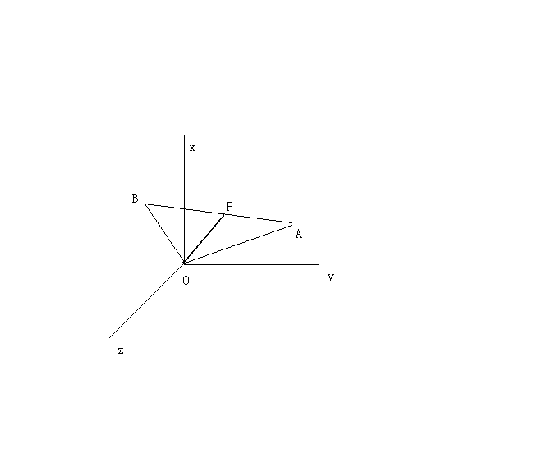
\includegraphics[scale=0.6]{gto.eps}\label{BASIS:1}
      \caption{the center theorem related to GTO}
    \end{center}
  \end{figure}

  If there's two center GTO orbital, one is residing on A, and the
  other is residing on B; we can prove that the multiplication of the
  two GTOs can be transformed into a one center of GTO, who is located
  in center of P (see the \ref{BASIS:1}).

  Thus we have:
  \begin{equation}\label{}
    exp(-ar_{A}^{2})exp(-br_{B}^{2}) = Kexp(-ar_{p}^{2})
  \end{equation}

\end{comment}

%%%%%%%%%%%%%%%%%%%%%%%%%%%%%%%%%%%%%%%%%%%%%%%%%%%%%%%%%%%%%%%%%%%%%%%%%%
\section{Contracted Gaussian type orbitals}
%
% to use the gaussian function, people always to contract them
% together to form the basis sets.  what's the relation between GTO
% and basis sets?  how to contract them to form the basis sets?
% introduce the two different way of contracting: segmental and
% general way
%
Gaussian primitives are usually obtained from quantum calculations on
atoms (i.e. Hartree-Fock or Hartree-Fock plus some correlated
calculations, e.g. CI). Typically, the exponents are varied until the
lowest total energy of the atom is achieved. In some cases, the
exponents are optimized independently. In others, the exponents are
related to each other by some equation, and parameters in this
equation are optimized (e.g. even-tempered or "geometrical" and
well-tempered basis sets). The primitives so derived describe isolated
atoms and cannot accurately describe deformations of atomic orbitals
brought by the presence of other atoms in the molecule.  Basis sets
for molecular calculations are therefore frequently augmented with
other functions, which has smaller exponent and able to describe the
motion of electrons far away from the nucleus.

For molecular calculations, these gaussian primitives have to be
contracted, i.e., certain linear combinations of them will be used as
basis functions. The term contraction means "a linear combination of
gaussian primitives to be used as basis function".  Such a basis
function will have its coefficients and exponents fixed. The
contractions are sometimes called Contracted Gaussian Type Orbitals
(CGTO). For instance, there's a four s-type gaussian primitives used
to represent 1s orbital of hydrogen as:
\begin{multline}\label{}
  \varphi_{1s} = 0.50907N_{1}e^{-0.123317r^{2}} +
  0.47449N_{2}e^{-0.453757r^{2}} \\
  + 0.13424N_{3}e^{-2.01330r^{2}} + 0.01906N_{4}e^{-13.3615r^{2}}
\end{multline}
$N_{i}$ is a normalization constant for a given primitive. In the case
of gaussian primitives of type s it is equal to
$(2\alpha/\pi)^{\frac{3}{4}}$.

These primitives may be grouped in 2 contractions. The first
contraction contains only 1 primitive:
\begin{equation}\label{}
  \phi_{1} = Ne^{-0.123317r^{2}}
\end{equation}

3 primitives are present in the second contraction:
\begin{multline}\label{}
  \phi_{2} = N[0.47449N_{2}e^{-0.453757r^{2}} +
  0.13424N_{3}e^{-2.01330r^{2}} \\
  + 0.01906N_{4}e^{-13.3615r^{2}}]
\end{multline}

N is a normalization constant for the whole contraction.

In this case, 4 primitives were contracted to 2 basis functions. It is
frequently denoted as $(4s) \rightarrow [2s]$ contraction (some use
(4s)/[2s] notation). The coefficients in function $\phi_{2}$ are then
fixed in subsequent molecular calculations.

Obviously, the best results could be obtained if all coefficients in
gaussian expansion were allowed to vary during molecular
calculations. Moreover, the computational effort (i.e. "CPU time") for
calculating integrals in the Hartree-Fock procedure depends upon the
4th power in the number of gaussian primitives. However, all
subsequent steps depend upon the number of basis functions (i.e.
contractions). Also, the storage required for integrals (when Direct
SCF is not used) is proportional to the number of basis functions (not
primitives!). Frequently the disk storage and not the CPU time is a
limiting factor. The CPU time requirements are more acute when
post-Hartree- Fock (e.g. correlated methods) are used, since the
dependance upon the number of basis functions here is more steep than
the 4th power.

There are two basic forms of contractions, namely "segmented" and
"general". The segmented contractions are disjointed, i.e., given
primitive appears only in one contraction. The example given above
$(4s) \rightarrow [2s]$ is a segmented contraction. Occasionally, one
or two primitives may appear in more than one contraction, but this is
an exception to the rule. The general contractions, on the contrary,
allow each of the primitives to appear in each basis function
(contraction). The segmented contractions are far more popular and
will be described first. The reason for their popularity is not that
they are better, but simply, that the most popular ab initio packages
do not implement efficient integral calculations with general
contractions. The computer code to perform integral calculations with
general contractions is much more complex than that for the segmented
case.

%%%%%%%%%%%%%%%%%%%%%%%%%%%%%%%%%%%%%%%%%%%%%%%%%%%%%%%%%%%%%%%%%%%%%%%%%
\subsection{Segmented basis sets}
%
% how to form the segmented basis sets? there's some rules: 1 the
% inner part is assigned with less flexibility (less basis sets), but
% more GTO used to get a better shape (such as 6-31g, use 6 GTOs to
% simulate the inner shell, but only three the the outer ones) 2 the
% outer ones are assigned with better flexibility (more basis sets) so
% that to make the basis sets more adaptable to the change of
% molecular environments.  3 also the polarized function and diffuse
% functions are used. they are always left uncontracted, since that
% they are not derived from the atom calculation.  these functions are
% used to help the basis set to change more flexible.
%
The segmented basis sets are usually structured in such a way that the
most diffuse primitives (primitives with the smallest exponent) are
left uncontracted (i.e. one primitive per basis function). More
compact primitives (i.e. those with larger exponents) are taken with
their coefficients from atomic Hartree-Fock calculations and one or
more contractions are formed. Then the contractions are renormalized.

Cartesian gaussian primitives are grouped in shells corresponding to
the same value of angular momentum quantum number. Of course, these
shells should not be confused with electron shells (i.e. electrons
with the same principal quantum number: $K \rightarrow n=1$, $L
\rightarrow n=2$, etc.). So as to avoid the ambiguity, we use s-shell,
p-shell, d-shell, f-shell, g-shell, etc. to signal the shell of
gaussian primitives. The shell is a collection of cartesian gaussian
primitives that have the same L (see definition of cartesian gaussian
above). Strictly speaking, the s-shell is a collection of s type
gaussian primitives; p-shell is a collection of p-type gaussian
primitives; d-shell is a collection of d-type gaussian primitives; and
so on. Of course, combining primitives belonging to different shells
within the same contraction does not make sense because primitives
from different shells are orthogonal.

But even here there is a room for more confusion. Many basis sets use
the same exponents for functions corresponding to the same principal
quantum number, i.e., electronic shell. 3-21g is an example, as well
as other basis sets from Pople's group. Atoms of the first and second
row (i.e. Li - Ne, Na - Cl) have the same exponents for s- and p-type
gaussian primitives formally associated with a given electron shell of
the isolated atom. For the basis sets in which s- and p-type functions
share the same exponents, the term SP-shell is used (here in the
output job file by Gaussian03, this is clearly
demonstrated). Sometimes term L-shell is used by analogy to the 2nd
electron shell. This approximation works very well in
practice. Moreover, it is possible to write efficient code for
calculating integrals for such cases. It is important to stress here
that the distinction between inner orbitals and valence orbitals is
kind of carry-over from the past era of Slater orbitals.  Contractions
consisting of primitives with large exponents are associated with
inner atomic orbitals while more diffuse functions are allied with
valence orbitals. Basis functions are not usually atomic orbitals, and
in many cases, they do not even resemble orbitals of isolated
atoms. In fact, examining coefficients of molecular orbitals
frequently reveals that these "core" basis functions contribute
substantially to the Highest Occupied Molecular Orbital (HOMO). It
comes as a consequence of the fact that basis functions on a given
center are usually not orthogonal to each other and "core" basis
functions on different centers overlap to a great extent - situation
not likely to occur with true atomic orbitals.

The early gaussian contractions were obtained by a least square fit to
Slater atomic orbitals. The number of contractions (not primitives!)
used for representing a single Slater atomic orbital (i.e. zeta) was a
measure of the goodness of the set. From this era we have terms like
single zeta (SZ), double zeta (DZ), triple zeta (TZ), quadruple zeta
(QZ), etc. In the minimal basis set (i.e. SZ) only one basis function
(contraction) per Slater atomic orbital is used. DZ sets have two
basis functions per orbital, etc. Since valence orbitals of atoms are
more affected by forming a bond than the inner (core) orbitals, more
basis functions are assigned frequently to describe valence
orbitals. This prompted development of split-valence (SV) basis sets,
i.e., basis sets in which more contractions are used to describe
valence orbitals than core orbitals. That more basis functions are
assigned to valence orbitals does not mean the valence orbitals
incorporate more primitives.  Frequently, the core orbitals are long
contractions consisting of many gaussian primitives to represent well
the "cusp" of s type function at the position of the nucleus. The
"zeta" terminology is often augmented with a number of polarization
functions which will be described later. So, DZP means double-zeta
plus polarization, TZP stands for triple-zeta plus polarization,
etc. Sometimes the number of polarization functions is given,
e.g. TZDP, TZ2P, TZ+2P stands for triple-zeta plus double
polarization. Letter V denotes split valence basis sets, e.g., DZV
represents basis set with only one contraction for inner orbitals, and
two contractions for valence orbitals. The creativity here is enormous
and spontaneous.

The minimal basis set is the smallest possible set, i.e., it contains
only one function per occupied atomic orbital in the ground
state. Actually, it always includes all orbitals from partially
occupied sub shells and valence p-type functions for elements from the
first 2 groups of the periodic table. So for Li and Be atoms it has 2
s-type contractions and 1 p-type contraction. Minimal basis set for S
atom has 3 s-type contractions and 2 p-type contractions.  The most
popular minimal basis sets are the STO-nG, where n denotes number of
primitives in the contraction. These sets were obtained by least
square fit of the combination of n gaussian functions to a Slater type
orbital of the same type with zeta = 1.0, For this set additional
constraint is used, that exponents of corresponding gaussian
primitives are the same for basis functions describing orbitals with
the same principal quantum number (e.g. the same primitives are used
for 2s and 2p function).For the minimal basis set, the STO-3G (i.e. 3
primitives per each function) is the most widely used set.

For other sets a more complicated notation needs to be used to specify
the number of primitives and contractions explicitly. The parentheses
() embrace the number of primitives that are given in the order of
angular momentum quantum number. Square brackets [] are used to
specify the number of resulting contractions. For example: (12s,9p,1d)
means 12 primitives on s-shell, 9 primitives on p-shell, and 1
primitive on d-shell. This is sometimes abbreviated even further by
skipping the shell symbols (12,9,1). The [5,4,1] means that s-shell
has 5 contractions, p-shell has 4 contractions and d-shell has 1
contraction. To denote how contractions were performed, the following
notation is frequently used: $(12,9,1) \rightarrow [5,4,1]$ or
$(12,9,1)/[5,4,1]$ or $(12s,9p,1d) \rightarrow [5s,4p,1d]$. This means
that 12 s-type primitives were contracted to form 5 s-type
contractions, 9 p-primitives were contracted to 4 basis functions and
1 d-primitive was used as a basis function by itself. Note of caution
here. The statement "9 p-primitives were contracted to 4 basis
functions" actually means that 12 basis functions were created. Each
p-type basis functions has 3 variants: $p_{x}, p_{y}, p_{z}$ which
differ in their cartesian part (i.e., angular part). The same is true
for d-, f-, and higher angular momentum functions.

%%%%%%%%%%%%%%%%%%%%%%%%%%%%%%%%%%%%%%%%%%%%%%%%%%%%%%%%%%%%%%%%%%%%%%%%
\subsection{Basis sets in computation}
%
% 1 importance in the understanding of the quantum chemistry codes 2
% introduce the primitive shells, and to see the difference between
% the gaussians and the primitive shells.  3 basis sets are linear
% combination of the primitive shells 4 shells concept 5 what should
% be contained in the quantum chemistry program
%
%
To some extent, basis sets is the foundation of the codes in the
quantum chemistry, it's impossible to understand any quantum chemistry
codes without the understanding of the basis sets. Hence, in this
section we hope to give some basic concept of how to express the basis
sets in the quantum chemistry codes. Here the examples are all from
the Gaussian program, but other programs share the similar ideas so
that it's easy to derive the others forms.

In the quantum chemistry program, it's a trivial way to store all the
basis sets information by the form of gaussian functions, in the
context below; we can see that it's some way too verbose. On the
contrary, it's convenient to contract the information inside the
gaussian functions to form some "compact" expressions, they are more
suitable to store in the computer and the information is easy to
extract from them. That's what we called the shells and the primitive
shells.

The primitive shells are defined as the set of gaussian functions
which share the same exponents and the same maximum quantum angular
number. For example, the $2s$, $2px$, $2py$ and $2pz$ are considered
to be the same primitive shell, but $1s$, $3d$ gaussian functions are
not in this primitive shell because they have different angular part.

Since that the $S$ type gaussian and $P$ type gaussian are always to
be made to share the same primitive shell, should we follow the same
way to deal with the $D$ orbital and even $F$ orbitals? But there's an
problem; that if people want to calculate the molecules containing the
$d$ orbitals; all the $S$, $P$ and $D$ gaussian functions in the same
shell will be introduced together (if the $d$ orbital is introduced as
some polarized functions, we do not want to do the work in this way);
thus some way need to devised to avoid this situation.

Therefore, for the higher angular momentum part of gaussian functions
(namely the $d$ type and the $f$ type), we use the constraint shells
instead; that is in these shells, only the $d$ or $f$ functions are
inside to form the primitive shells. The only difference related to
these shells is only that to use the pure form or the cartesian
form. For the $d$ type of orbitals, the pure type owns only five
orbitals, whereas the cartesian type has six orbitals; these has been
discussed in the above content.

In the real program, so far people always use the the $SP$ shell to
represent the $s$ type and $p$ type gaussians (thus they share the
same exponents), this is popular in the Pople basis sets; but in other
kind of basis sets such as the Dunning basis sets, the $s$ and $p$ are
separated to be into different primitive shells.

At last let's give some example. Take the oxygen atom of the $6-31g$
as an example, the $6$ gaussians are the six primitive shells (they
have different exponents), they are composed into the basis function
which characterizes the inner orbital of $1s$. On the other hand, the
other $3$ gaussians and additional one gaussians form the other two
group of primitive shells, each one represents the $2s$, $2px$, $2py$
and $2pz$, separately. Thus the ten primitive shells represents $9$
basis sets and contain $14$ gaussian functions.

Now we can see that if we use the pure gaussian functions instead,
it's some too wordy way since that different $px$ $py$ and $pz$ are
take into account. Therefore, in the quantum chemistry the primitive
shells are used as the elementary brick to construct the storing whole
basis sets.

Next, the basis sets are considered to be the linear combination of
the same type of the primitive shells. Thus the basis sets consist of
the same type of angular part. In quantum chemistry, the basis sets is
the most elementary components, the function space are formed from the
variation of the basis sets.

Finally, shells are the most abstract concept. The shell is considered
to contains the same type of primitive shells, they share the same
angular momentum number. For example, $S$ shell, $P$ shell or $D$
shell. It can see that the concept of shell is larger than the basis
sets. For example, the basis of $6-31g$ use two different basis sets
to represent the same type of shell (if for oxygen atom, it's the $SP$
shell; if for the $Br$ atom, it's the $3d$, $4s$ and $4p$ shell).

At last, we try to list the data information used in the common
quantum chemistry package. All the basis sets information, is actually
contracted into the shell array (also the primitive shell array). Here
below is the necessary part of these arrays:
\begin{itemize}
\item for each shell, what kind of atom it belongs to.
\item for each shell, the starting point of its gaussian functions
  list. For example, O atom with $6-31g$ basis set has three shells
  $(1s, 2sp, 3s^{'}p^{'})$. $1s$ has six primitives, thus $array(1) =
  1$, $array(2) = 7$. In this way we can determine the number of
  gaussians it contains.
\item the number of gaussians for each shell.
\item for each shell, what is its angular part? $S$, $SP$ or $D$?
\item For the $D$ or $F$, we use the pure ones or cartesian ones?
\item total shell number
\item the maximum angular type
\item the exponent array, and the corresponding coefficients for the
  primitive shells
\end{itemize}

%%%%%%%%%%%%%%%%%%%%%%%%%%%%%%%%%%%%%%%%%%%%%%%%%%%%%%%%%%%%%%%%%%%%%%%%%%
\subsection{Pople's Basis Sets}
A different convention was adopted by Pople and coworkers. The basis
set structure is given for the whole molecule, rather than particular
a atom. This notation emphasizes also a split valence (SV) nature of
these sets. Symbols like n-ijG or n-ijkG can be encoded as: n - number
of primitives for the inner shells; ij or ijk - number of primitives
for contractions in the valence shell. The ij notations describes sets
of valence double zeta quality and ijk sets of valence triple zeta
quality. Generally, in basis sets derived by Pople's group, the s and
p contractions belonging to the same "electron shell"
(i.e. corresponding formally to the same principal quantum number n)
are folded into a sp-shell. In this case, number of s-type and p-type
primitives is the same, and they have identical exponents. However,
the coefficients for s- and p-type contractions are different.

Now, we are giving some examples. The 4-31G basis set for hydrogen
(hydrogen has only valence electrons!) is a contraction $(31)$ or
$(4s)\rightarrow[2s]$; for first row atoms $(8s,4p) \rightarrow
[3s,2p]$; and for 2nd row atoms the contraction scheme is $(12s,8p)
\rightarrow [4s,3p]$. The 6-311G set represents the following
contractions for water is $(11s,5p/5s) \rightarrow [4s,3p/3s]$.

The Pople's basis sets can also be augmented with d type polarization
functions on heavy atoms only (n-ijG* or n-ijkG*) or on all atoms,
with p-functions on hydrogens (n-ijG** or n-ijkG**). In methane, the
4-31G* encodes following split $(8s,4p,1d/4s) \rightarrow
[3s,2p,1d/2s]$, while 6-311G** for HCN molecule would involve
following contractions: $(11s,5p,1d/5s,1p) \rightarrow
[4s,3p,1d/3s,1p]$.




%%% Local Variables:
%%% mode: latex
%%% TeX-master: "../../main"
%%% End:
